\documentclass{sigchi}

% Use this command to override the default ACM copyright statement (e.g. for preprints).
% Consult the conference website for the camera-ready copyright statement.


%% EXAMPLE BEGIN -- HOW TO OVERRIDE THE DEFAULT COPYRIGHT STRIP -- (July 22, 2013 - Paul Baumann)
% \toappear{Permission to make digital or hard copies of all or part of this work for personal or classroom use is 	granted without fee provided that copies are not made or distributed for profit or commercial advantage and that copies bear this notice and the full citation on the first page. Copyrights for components of this work owned by others than ACM must be honored. Abstracting with credit is permitted. To copy otherwise, or republish, to post on servers or to redistribute to lists, requires prior specific permission and/or a fee. Request permissions from permissions@acm.org. \\
% {\emph{CHI'14}}, April 26--May 1, 2014, Toronto, Canada. \\
% Copyright \copyright~2014 ACM ISBN/14/04...\$15.00. \\
% DOI string from ACM form confirmation}
%% EXAMPLE END -- HOW TO OVERRIDE THE DEFAULT COPYRIGHT STRIP -- (July 22, 2013 - Paul Baumann)


% Arabic page numbers for submission.
% Remove this line to eliminate page numbers for the camera ready copy
% \pagenumbering{arabic}


% Load basic packages
\usepackage{balance}  % to better equalize the last page
\usepackage{graphics} % for EPS, load graphicx instead
\usepackage{times}    % comment if you want LaTeX's default font
\usepackage{url}      % llt: nicely formatted URLs

%my pachages
\usepackage{framed}
\usepackage{listings}
\usepackage[]{algorithm2e}

% llt: Define a global style for URLs, rather that the default one
\makeatletter
\def\url@leostyle{%
  \@ifundefined{selectfont}{\def\UrlFont{\sf}}{\def\UrlFont{\small\bf\ttfamily}}}
\makeatother
\urlstyle{leo}


% To make various LaTeX processors do the right thing with page size.
\def\pprw{8.5in}
\def\pprh{11in}
\special{papersize=\pprw,\pprh}
\setlength{\paperwidth}{\pprw}
\setlength{\paperheight}{\pprh}
\setlength{\pdfpagewidth}{\pprw}
\setlength{\pdfpageheight}{\pprh}

% Make sure hyperref comes last of your loaded packages,
% to give it a fighting chance of not being over-written,
% since its job is to redefine many LaTeX commands.
\usepackage[pdftex]{hyperref}
\hypersetup{
pdftitle={SIGCHI Conference Proceedings Format},
pdfauthor={LaTeX},
pdfkeywords={SIGCHI, proceedings, archival format},
bookmarksnumbered,
pdfstartview={FitH},
colorlinks,
citecolor=black,
filecolor=black,
linkcolor=black,
urlcolor=black,
breaklinks=true,
}

% create a shortcut to typeset table headings
\newcommand\tabhead[1]{\small\textbf{#1}}


% End of preamble. Here it comes the document.
\begin{document}

\title{JobFinder: A Personalized Resume-Job Matching System}

\numberofauthors{3}
\author{
  \alignauthor 1st Author Name\\
    \affaddr{Affiliation}\\
    \affaddr{Address}\\
    \email{e-mail address}\\
    \affaddr{Optional phone number}
  \alignauthor 2nd Author Name\\
    \affaddr{Affiliation}\\
    \affaddr{Address}\\
    \email{e-mail address}\\
    \affaddr{Optional phone number}
  \alignauthor 3rd Author Name\\
    \affaddr{Affiliation}\\
    \affaddr{Address}\\
    \email{e-mail address}\\
    \affaddr{Optional phone number}
}

\maketitle

\begin{abstract}
Today, online recruiting web sites such as Monster and Indeed have become one of the main channels for people to find jobs. These web platforms have provided their services for more than ten years, and have saved a lot of time and cost for both job seekers and organizations who want to hire people. However, traditional information retrieval techniques may not be appropriate for users. The reason is because the number of results returned to a job seeker may be huge, so job seekers are required to spend a significant amount of time reading and reviewing their options. One popular approach to resolve this difficulty for users are recommender systems, which is a technology that has been studied for a long time.

In this paper we have made an effort to propose a personalized job-resume matching system, which could help job seekers to find appropriate IT jobs more easily.  We create a finite state transducer based information extraction library to extract models from resumes and job descriptions. We devised a new Statistical-based ontology similarity measure to compare the resume models and the job models. Since the most appreciate jobs will be returned in front of other jobs, the users of the system could get better result than current job finding website. To evaluate the system, we had compared NDCG of the job searching results of the system to other classic information retrieval approaches, and the result showed that the system has obvious advantage than those approaches
\end{abstract}

\keywords{
User Interfaces; Recommender Systems; Semantic Web; Information Retrieval
}

\category{H.5.m.}{Information Interfaces and Presentation (e.g. HCI)}{Miscellaneous}

See: \url{http://www.acm.org/about/class/1998/}
for more information and the full list of ACM classifiers
and descriptors. \newline
\textcolor{red}{Optional section to be included in your final version,
but strongly encouraged. On the submission page only the classifiers��
letter-number combination will need to be entered.}


\section{Introduction}

Currently, the main channel for job seekers are online job finding web sites, such as Indeed or Monster, that make the job finding process easier and reduce the recruitment time. However, most of these web sites only allow users to use keywords to search for jobs, which makes job searching both tedious and random. For example, if a user types the keyword ``java'' to search for jobs with locations restricted to Mountain View in California on job search site indeed.com, then the web site would return approximately 7,000 jobs. While the number of job search results is huge, it is also not ranked in order of relevancy, so the job seeker has to manually review every job description. Since an individual does not have the time to read over all the jobs in the search result, the actual quality of the job searching service is low. This is a classic problem of information overflow.

The reason for such results is because current job searching web sites use the same type of information retrieval technology like ``Inverted index'' \cite{zobel2006inverted} that are generally used in their search engines, which just rely on keywords to map all the stored documents. Current search engines all use some sort of ranking algorithms to sort these search result, like page rank \cite{page1999pagerank}, so the top results are the most related ones. But such algorithms are unavailable to the job searching systems, because the criteria  of how to rank the job searching result is very personalized. A great job opening for one job seeker may not look as good to someone else, because the goodness of a job to a different job seeker heavily depends on their personal background, like their education or professional experience and so on.

Since people's resumes contain their most important background information, we believe the content of the resume could be used to rank the job openings. We propose an online system that could use the resumes of job seekers to find the jobs that best match their profiles. The main idea is to calculate the similarity between the candidate model and job models, which should be generated from resumes and job descriptions. An important goal of the research is therefore to transfer the job searching task from keywords searching to job and resume models matching. The matching result will be sorted by the matching score, where the higher matching score means a better matching. The matching algorithm will not only help job seekers find the appreciate job opening, but will also offer priority to them~\cite{gueutal2006brave}. We hope the job matching process could help job seeker search and rank the job opening, and save them some time.

\subsection{Contribution}

We had made three key contributions in this work. The first is creation of a Finite State Transducer-based matching tool, which is a lightweight and flexible library, can be extend in very easy ways. The second is is the introduction of a semi-automatic approach, which could collect technical terms from data sources. The third contribution is a statistical based Ontology similarity measure for comparing the job seeker's resumes and job descriptions.

\section{Related Works}
This section provides a discussion of related research in Job Recommender Systems.

\subsection{Job Recommender Systems}

Recommender Systems are sfotware tools and techniques providing suggestions for items to be of use to a user~\cite{ricci2011introduction}.

Rafter et al. \cite{rafter2000personalised} began to use ACF (Automated Collaborative Filtering) in their Job Recommender system, ``CASPER''. In the system user profiles are gotten from server logs, that included: revisit data, read time data, and activity data. All these factors were viewed as measure of relevance among users. The system recommend jobs in two steps. First the system find a set of user related to the target user, second the jobs that related users liked will be recommend to the target user. The system use cluster-based Collaborative Filtering strategy. The similarity between users are based on how many jobs they both reviewed, or applied.

The shortage of Collaborative Filtering:
 First since the searching result is huge, and the result is sorted randomly, even two very similar users may review different jobs,  or say the probability of two similar users reviewing the same job is low. The authors also noticed the such sparseness problem in users profile, so they try to user cluster-based solution to resolve this problem.

 Second because recommended jobs are from others users searching result, since the current quality of current searching result is low, so the quality of recommendation cannot be high.

F{\"a}rber et al \cite{farber2003automated}. presented a recommender system built on a hybrid approach. The system integrated two methods, content-based filtering and collaborative filtering. They tried to overcome the problem of rating data sparsity by leveraging synergies of a combined model, et. the  latent aspect model.

Daramola et al.  proposed a fuzzy logic based expert system(FES) tool for online personnel resctuitments. In the paper, the authors assumed that the information already be collected. The system use a fuzzy distance metric to rank candidates' profile in the order of their eligibility for the job. The fuzy hamming distance is given as:
$$ \delta \left ( O,R \right )=\sum_{i=1}^{n}\left | \mu_O(x_i) - \mu_R(x_i)  \right | $$


when applying a job, the common method is let the candidates upload their resumes, sometimes the company want user to enter details like personal information, education and experience details, skills. However, in real life, the candidates do not input a lot information in the on-line form. ~\cite{singh2010prospect}

\subsection{Information Extraction}

The content-based recommender systems need the structured information of items. But the items in JRS are resumes and job descriptions written in natural language, so how to get information from the documents is an important problem. Information extraction (IE) is the task of automatically extracting structured information from unstructured and/or semi-structured machine-readable documents.

Amit et al. in IBM presented a system, ``PROSPECT'', ~\cite{singh2010prospect} to aid in the shortlisting of candidates for jobs. The system uses a resume miner to extract the information from resumes, which use a CRF model to segment and label the resumes. The CRF model used three kinds of features, they are: Lexicon, Visual, Named Entity, Text, and Conjunction. The paper compared some algorithms to ranked the candidates applicants, such methods include: Okapi BM25, KL, Lucene Scoring, and Lucene Scoring + SkillBoost.

HP also built a system to solve the similar problem, which was introduced in Gonzalez et al.'s paper ~\cite{gonzalez2012adaptive}. The system also pay a lot of attention to information extraction.

Yu et al.~\cite{yu2005resume} used a cascaded information extraction (IE) framework to get the detailed information from the job seeker��s resume. In the first stage, the Hidden Markov Modeling (HMM) model is used to segment the resume into consecutive blocks. Based on the result, a SVM model is used to obtain the detailed information in the certain block, the information include: name, address, education etc.

 Celik Duygua and Elci Atilla proposed a Ontology-based R��sum�� Parser (ORP) ~\cite{ccelik2013ontology}, which uses ontology to assistant the information extraction process. The system process the resume in following steps: convert the resume files into plain text, separate the text into  some segments, use Ontology Knowledge Base to find the concepts in the sentences, normalize all the terms, at last the system will classify the sentences to get the wanted terms.

\subsection{Ontology-based Approaches}

A domain-oriented ontology is used to represent knowledge, inference rules are defined based on the ontology knowledge base. When a detected term found, the system will search in external knowledge base, like DBpedia etc. The resume also be classified to different categories like ``Web Technology'' and ``No Web Technology'' by naive Bayes classifier. The company could allocate appropriate employees to required positions.
The Ontology technics had also been used in some JRSs, which provide a formal specification of a shared conceptualization~\cite{guarino1998formal}.

Yao et al.~\cite{lu2013recommender} also presented a hybrid recommender system which integrated content-based and interaction-based relation. In content-based part, relations between job-job, job-job seeker, and job seeker - job seeker could be identified by their similarity of profiles.

This system was build on the assumption: The users with similar profiles tend to have similar interests. But here we could find two problems: At first, people with similar profile may not have similar interest, this is a very common fact. For example two students both graduate from same department with the same degree at the same year, when they look for jobs, they may have different preference. Second, to job's part, the accuracy of similarity calculation will effect a lot on the result of the system, since two very similar job may be classified as different jobs in the system.

\section{System Overview}
The system will use rule based information extraction technique to parse the job description and resume, and get information such as skill, specialties and background. These information will be used to create the model of job description and job seeker.  Ontology will be used to construct the knowledge base, which will include the taxonomy and rules, to support resume-job matching.

The model of candidates will include their specialties, working experience and education background, all the them should be extracted from the resumes. The job model will be extracted from job description, the information will include: company name, location, job title, education requirement, skill requirements and working experiences etc. When a job seeker searches the jobs by his resume, the system will calculate the similarity between the candidate model and the job models, give every job model a similarity score.

User��s personal preference should be considered as well. In the previous user survey, some factors will impact a lot on the user��s expectation of good jobs, such factors include: location, the reputation of the company, the salary etc. These factors will be treated as weight factors in the job matching algorithm.

\subsection{System Architecture}

The architecture of the system is shown in Figure ~\ref{fig:Pipeline}, which includes several modules:

\begin{enumerate}
    \item The web crawler could search and download all new IT job opening web pages  from indeed.com everyday.
    \item The job parser could parse the job opening web page, extract the information and create the job model.
    \item The resume Parser is much like the Job parser, it will parse the resume and create the candidate model.
    \item All the job models will be stored in the Job Description database.
    \item When user makes a match request, the ontology matcher will calculate the matching score of each job, and return the jobs ranked by the scores.
\end{enumerate}

\begin{figure}[htbp]
  \centering
  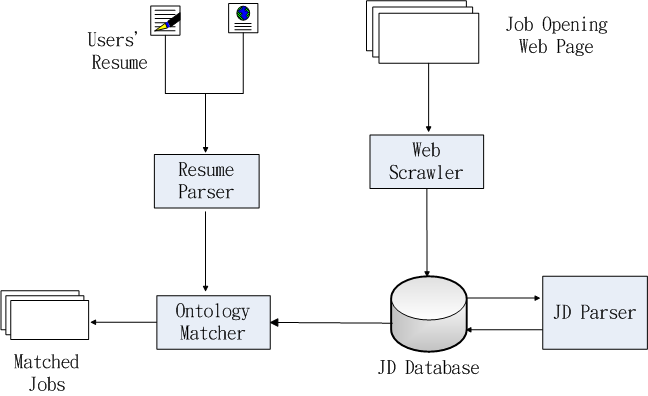
\includegraphics[scale=0.35]{images/arch.png}
  \caption{System Architecture}
  \label{fig:arch}
\end{figure}

\section{Information Extraction}

To create the models from Job Descriptions and Resumes, the system need to extract information from resumes and job descriptions. Both resumes and job descriptions are written in natural language, so the challenge is how to extract information from such unstructured or semi-structured data source, and transfer them to some designed structure.

\subsection{Text Processing Pipeline}

In Nature Language Processing, especially in Information Extraction, pipeline is a well adopted architecture~\cite{sarawagi2008information}. This pipeline to process the job descriptions in the system has eight stages, which is shown in Figure~\ref{fig:Pipeline}:

\begin{enumerate}
    \item The HTML parser will parse the web pages of job descriptions, which are obtained from web crawler. The parser will get the HTML element that contains the main content of the job description.
    \item Segment module will separate the job description into paragraphs according to HTML tags at first, then separate each paragraph into sentences.
    \item The sentences will be tokenized into string arrays, and be sent to the classification module. The classification module will determine the category of the sentence, and the sentence a category mark.
    \item The preprocessing module will delete unreadable characters, and correct some tokens spelling.
    \item The annotation module will annotate the tokens with semantic and ontology labels. After labeling, the sentences will have a multi-layered data structure.
    \item The layered sentences will be matched with pre-defined patterns with the FST library. If any pattern could be matched, the ontology information will be extract and stored in the job model.
    \item After every sentence has be processed in the pipeline, the job model will be stored into database.
\end{enumerate}


\begin{figure}[htbp]
  \centering
  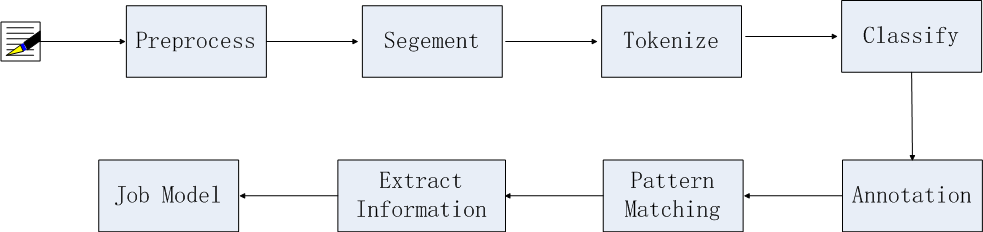
\includegraphics[scale=0.25]{images/pipeline.png}
  \caption{Job Description Process Pipeline}
  \label{fig:Pipeline}
\end{figure}


\subsection{Regular Expression Over Tokens}
There is two completive techniques in Information Extraction, one is machine learning-based approach, the other is rule-based approach. Chiticariu et al. \cite{chiticariu2013rule}summarized the pros and cons of machine learning (ML) and rule-based IE technologies. In this work, we prefer the rule-based approach because:
\begin{enumerate}
    \item Most of sentences that contain the information share some common patterns that can be easily identified.
    \item A lot of sentences are not grammatical completed as a sentence, for example some of them missing subject, and some of them are just a list of terms.
    \item Processing speed is also a concern, and generally rule-based approach is faster.
\end{enumerate}

Cascaded Finite-State Transducer as a tool to match patterns and extract information for more than 20 years. It has been demonstrated very effective in extracting information from text in the systems like in CIRCUS~\cite{lehnert1991university} and FASTUS~\cite{hobbs199713}.   JAPE (Java Annotations Pattern Engine), the key component of the widely used NLP toolkit GATE~\cite{cunningham2002framework}, can describe patterns and annotations with its domain-specific language (DSL).  JAPE adopted a version of CPSL (Common Pattern  Specification Language)~\cite{appelt1998common}, which provides finite state transduction over annotations. Chang et al. proposed another tool for cascaded regular expressions over tokens~\cite{chang2014tokensregex}, which can define and matching patterns over token sequences.

After studying these tools, we found most them are powerful, complex, but not very flexible. Because at first, developers need to learn some DSLs like CPSL, and second to integrate the pattern matching tool in  into the system need extra efforts. So here we proposed a more flexible and lightweight framework, which can do regular expression matching over labeled tokens. The difference between this library and regular expression is that the basic unit to be matched is token, not character. In the library, a pattern is a concatenation of matchers�� which can match a single token, or can be a wrapper of other matchers. Currently we support seven types of matchers, those are listed in table~\ref{tab:matchers}.

\begin{table}[ht]
\small
\caption{Matcher Class } % title of Table
\centering % used for centering table
\begin{tabular}{  | p{2cm} | p{3cm} | p{3cm} |  }
 \hline
 Class Name        &  Function                                 & Counter Part of Regex       \\
  \hline
 UnitMatcher       &  token is matches the it                  & character  in regex       \\
 \hline
 SequenceMatcher   &  A list of Matcher                        & sequence of characters       \\
  \hline
 QuestionMatcher   &  One or more of the preceding token       & ?       \\
  \hline
 StarMatcher       &  Zero or more of the preceding token      & *       \\
  \hline
 PlusMatcher       &  Zero or one of the preceding token       & +       \\
  \hline
 DotMatcher        &  Any token                                & .      \\
  \hline
 RegexMatcher      &  Any token matches the regular expression               &        \\
  \hline

\end{tabular}
\label{tab:matchers} % is used to refer this table in the text\section{Pipeline of Information Extraction}
\end{table}

The framework support three styles to create patterns, which gives developers big flexibility. The most common style is define pattern expression in a string, which is much like traditional regular expression. We give an example as follows:

\begin{framed}
\small
\begin{lstlisting}[language=Python]
seqMatcher =parser.parse("aaa | bbb ccc? * ddd")
\end{lstlisting}
\end{framed}

The seconde style is using algebra operator to connect matchers, as follows:
\begin{framed}
\small
\begin{lstlisting}[language=Python]
seqMatcher =  TokenMatcher("aaa") +
    TokenMatcher("bbb") | TokenMatcher("ccc")
\end{lstlisting}
\end{framed}

We also could create complex matcher in programming style, which like we create and use some objects when programming, like this:

\begin{framed}
\small
\begin{lstlisting}[language=Python]
matcher1 = TokenMatcher("aaa")
matcher2 = TokenMatcher("bbb")
matcher3 = TokenMatcher("ccc")
matcher4 = AlternateMatcher([matcher1,matcher2])
seqMatcher = SeqMatcher([matcher3,matcher4])
\end{lstlisting}
\end{framed}


\subsection{Semantic Labeling}

In the text of natural language, one concept always have some different expressions. Like bachelor's degree, the simple concept has several expression in job descriptions, like B.S., BA/BS, 4 years degree, and so on. We list the words that if followed with word "degree", have the meaning ``bachelor's degree'' is shown is table ~\ref{tab:multispelling}:

\begin{table}[ht]
\caption{All words have meaning bachelors } % title of Table
\centering % used for centering table
\begin{tabular}{  | p{8cm} |  }
 \hline
 "Baccalaureate","bachelors", "bachelor" ,"B.S.", "B.S","BS","BA","BA/BS", "BABS", "BSBA", "B.A." ,"4-year","4-year", "4 year", "four year","college","Undergraduate" , "University" \\
  \hline
\end{tabular}
\label{tab:multispelling} % is used to refer this table in the text\section{Pipeline of Information Extraction}
\end{table}


The regular expression over tokens is a finite state machine (FSM) with states that are the tokens need to be matched with. If all above words are added to the regular expression, the FSM will have too many states, and the matching process will be very slow because of the problem of combinatorial explosion.

To resolve this problem, we proposed an approach to use the patterns match the semantic label of the sentences, not the the original text. Because in this system, we don't care what the words the sentences really use, we want to extract the semantic value from the matching phrases. 

We propose a two layers labeling approach. In the first layer, we labeled the word with its semantic meaning, which is the value that we want to extract from the sentence. In the second layer, the labels are the semantic categories of the first layer labels. For example the word "bachelors" will be labeled in the first layer with label "BS LEVEL", which means bachelors degree level, and the word "PhD" will be labeled as "PHD LEVEL". In the second layer, they both be labeled with "DEGREE LEVEL". A labeled sentence is shown in ~\ref{tab:labeldsent}.

\begin{table}[ht]
\small
\caption{Labeled sentence } % title of Table
\centering % used for centering table
\begin{tabular}{  | c | c | c | p{1cm} | c |c | c | p{1cm}  |  }
 \hline
  DE LEVEL   & DEGREE & IN & MAJOR            & OR & MAJOR   \\
 \hline
  BS LEVEL   & DEGREE & IN &  MAJOR CS        & OR &  MAJOR INFO      \\
 \hline
 bachelors   & degree & in & computer science & or & information systems      \\
  \hline
\end{tabular}
\label{tab:labeldsent} % is used to refer this table in the text\section{Pipeline of Information Extraction}
\end{table}

To resolve the problem of one concept with multiple expressions, we create a dictionary, in which the key is the different spellings an expressions, and the value is the meaning of the concept. For example the table ~\ref{tab:multispelling} shows all keys in the dictionary with and the values ``bachelors''.

After labeling, the sentence become a sequence of arrays, each array includes the token and its labels in two layers. The flexibility of the tool also comes from that developers could determine which layer of of array should be matched, the original text or labels in the first or second layer.  Developers can assign lambda expressions to the matcher's catching function, which defines how to get the matching input,  and out function, which defines what should be outputed. For example,  to match the labeled sentence, we set the lambda expression for catching function to "lambda x:x[2] ", and the out function to "lambda x:x[1]", which make the matcher match the pattern with the semantic category, and output the  the value of semantic value. We show some patterns used to match degree phases in table ~\ref{tab:patterns}:

\begin{table}[ht]
\small
\caption{Patterns match degree} % title of Table
\centering % used for centering table
\begin{tabular}{  | l  |  }
 \hline
 DE\_LEVEL,  DE\_LEVEL, OR  DE\_LEVEL DEGREE   \\
 DE\_LEVEL DEGREE ( IN  $\vert$  OF ) DT MAJOR   \\
 MAJOR\_DEGREE  ,  MAJOR\_DEGREE OR MAJOR \\
 DE\_LEVEL (, DE\_LEVEL)* (OR DE\_LEVEL)? BE? PERFER\_VBD   \\
 \hline


\end{tabular}
\label{tab:patterns} % is used to refer this table in the text\section{Pipeline of Information Extraction}
\end{table}


\section{Ontology Construction and Similarity}

We noticed that simple keywords matching is far from satisfied, because the same concepts could be written in different ways, and some different concepts have a close relationship. For example, Table~\ref{tab:resume_jd}  is part of the resume of a job seeker, and part of a job description:

\begin{table}[ht]
\caption{Resume and Job Description} % title of Table
\centering % used for centering table
\begin{tabular}{ | p{8cm} |  }
 \hline
   \textbf{Part of Resume}                  \\ \hline

    B.S. degree in computer science \newline
    5+ years Java \newline
    2+ year   C++  \newline
    Some experience in Oracle database \newline
    Other experience like: \newline
    Hibernate, JBOSS, JUnit, Tomcat etc. \\ \hline
 \hline
   \textbf{Part of Job Description} \\ \hline
  BS degree above   \newline
  4+ years Java  \newline
  Some experience of Python   \newline
    Mysql, MS-SQL   \newline
    Java web application Server   \newline
    OOA/OOD   \\
 \hline
\end{tabular}
\label{tab:resume_jd} % is used to refer this table in the text
\end{table}

If just looking at the text, we can find the resume has few common words with the job description.  But from the view of an experienced engineer, the candidate is pretty matching the job. Because relational databases Oracle and Mysql are very similar, OOA/OOD is the same meaning of many years of Java and C++ experience, and Tomcat and JBOSS are two Java web applications servers.  If we use keywords matching, the system won't give a good matching result in this very common situation. So we use ontology as a knowledge base to store all the relations of concepts, and a measurement of similarity between two concepts. 

\subsection{Ontology-based semantic similarity}

There are three kinds Ontology-based similarity measures have been studied, they are edge counting approaches, feature-based measures, and Measures based on Information Content. Rada, et al.,~\cite{rada1989development} measure the similarity by the distance of two nodes in the graph. 

\subsection{Statistical-based Ontology Similarity Measure }
 In most of job descriptions, they will list many skills the job required. From observation, we found that related skills always exist in a job description simultaneously, and the positions of them are always close, e.g. HTML and CSS are always required together, and appear in the same sentence. We could see this phenomenon in table~\ref{tab:skillinsent}, which include some skills requirement sentences from some job desertions. Based on such observation, we give a new statistical-based Ontology Similarity Measure. Two concepts can get similarity If the two concepts $a$ and $b$ have the same direct hypernym or one  is the hypernym of the other one, their similarity $S_{a,b}$ could be the ratio of two factors:

\begin{enumerate}
    \item The ratio of the number of documents they exist together $N_{a \cap b}$ to the number of documents have a least one them $N_{a \cup b}$.
    \item The average $\log$ value of their minimum distance $mindis(doc,a,b)$ in documents that have them both.
\end{enumerate}

$$ S(a,b) = \frac{  N_{a \cap b} / N_{a \cup b} }{avg(\log_2( mindis(doc,a,b) + 1 ))} $$

We set the restriction because the position of the concepts in the ontology are based on their technical similarity to others. Similar techniques will assigned into a same category, they should share the same technology base, and one could be a alternate or similar to the other. For example, we put EJB and Hibernate in the same category, because they are both J2EE persistence layer technologies, and both have the O/R mapping concept. If the applicant is familiar one of them, they can master the other very quickly. Another example, like Grail and Django, they are both web frameworks, and share some web design philosophies, but one is  designed for Java web application and the other is created for Python web application. So if one developer has some some experience with one of them, he/she still need spend a lot of time to learn the other to overcome the gap between programming languages. 


\subsection{Ontology Construction}

Semantic web have been a hot research topic in these years, thousands of domain ontologies had created~\cite{ding2004swoogle}. A paradigmatic example is WordNet~\cite{fellbaum1998wordnet}, is a general purpose thesaurus, that contains more than 100,00 general English concepts.  Currently, there is no IT technology ontology build for recruiting purpose.  ACM has created a poly-hierarchical ontology that can be utilized in semantic web applications~\cite{acm2012class}, but it is mostly used in academic area.

The IT ontology for recruiting should include a lot detailed information, like programming language, programming library, commercial products and so on. Furthermore there are new techniques invented everyday, so new IT terms will appear continuously. The task of creating such a ontology is a huge one. Ding et al.~\cite{ding2002ontology} give a survey of current ontology generation approaches, such as manual, semi-automatic, and automatic. Some aspects the approaches had been discussed in the paper, like the source data, concept extraction methods, Ontology representation, construction tools and so on.  Inspiring on this paper, we used semi-automatic approach to construct the IT skill ontology. We use Protege to create the skeleton of the ontology.

\begin{figure}[htbp]

  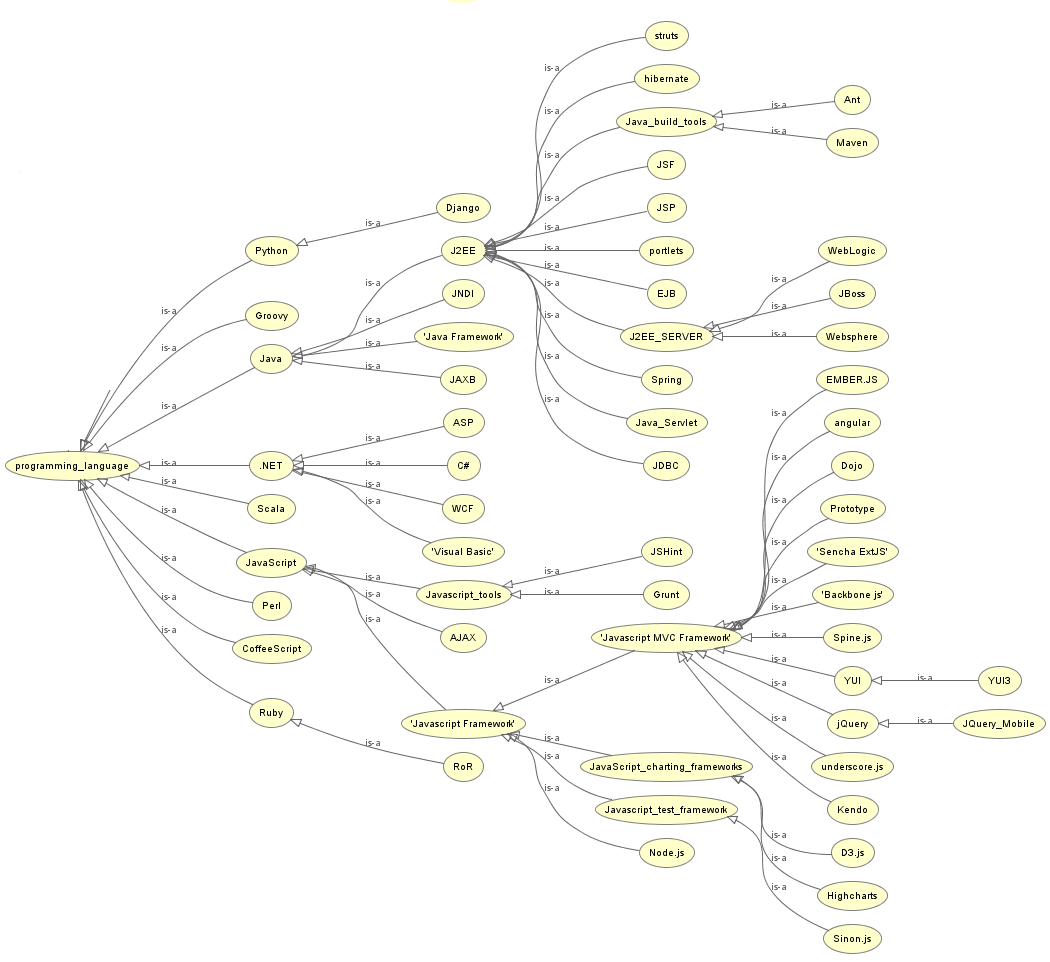
\includegraphics[scale=0.4]{images/ontology_pro.png}
  \caption{Part of Ontology}
  \label{fig:ontology_pro}
\end{figure}

We use semi-automatic approach to get the skills' terms from the job descriptions. From the observation, we found that  skills requirement part of job description always list several skills in one the sentence, which is shown in table ~\ref{tab:skillrequirement}.
\begin{table}[ht]
\caption{Some sentences Job Description} % title of Table
\centering % used for centering table
\begin{tabular}{ | p{8cm}  | }
 \hline
    1. A high-level language such as Java, Groovy, Ruby or Python; we use Java and Groovy extensively \newline
    2. HTML5/CSS3/JavaScript, web standards, jQuery or frameworks like AngularJS would be great \newline
    3. HTML CSS and Javascript a must  \newline
    4. Experience with AJAX, XML, XSL, XSLT, CSS, JavaScript, JQuery, HTML and Web Services   \\
 \hline
\end{tabular}
\label{tab:skillrequirement} % is used to refer this table in the text
\end{table}

Based on this character�� we propose a bootstrap approach to collect IT terms in job descriptions. We first manually collect about fifty terms in job descriptions, and add them to term dictionary. We use our pattern matching tools to find sentences matching some patterns like below, for example the sentence in ~\ref{tab:termspattern}, we could extract the words that matching *, they have high probability to be  terms. Then we could check the words in Dbpedia to if they are under the categories like software, programming language or any other technical related ones. If they are, we could classify them as terms.

$$ < term > , * , *, <term>$$
$$ < term > , * , *, and <term>$$

\begin{table}[ht]
\small
\caption{Some sentences Job Description} % title of Table
\centering % used for centering table
\begin{tabular}{   | c | c | c | c |c | c |c | c |c | c |c | c |c | c |  }
 \hline
     Experience & with & TERM & , & *   & , & *   &, & TERM &, & and & *  \\
 \hline
     Experience & with & AJAX & , & XML & , & XSL &, & XSLT &, & and & CSS  \\
 \hline
\end{tabular}
\label{tab:termspattern} % is used to refer this table in the text
\end{table}

For example, we extract the word  ''XSL'', which currently not in the skill set. We check the word on DBpedia, get the XML formatted description from URL : http://dbpedia.org/page/XSL. If the any of ``dcterms:subject'' fields have the value which is the technical category,  like ``Programming languages'', ``Markup languages'', we could indignity the word is a technical term, and pop them up. After getting a list of new terms, we could check the category of terms in Dbpedia, and put them into right position of our domain specific ontology. Such iteration will continue until the number of new terms getting below a threshold. The process is shown Figure ~\ref{fig:gen_onto}

\begin{figure}[htbp]
  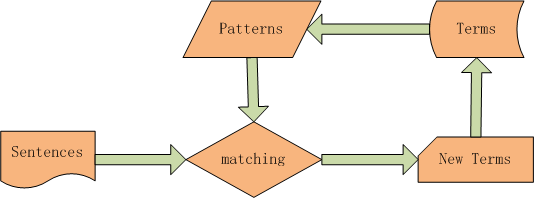
\includegraphics[scale=0.4]{images/genonto.png}
  \caption{Find Technical Terms}
  \label{fig:gen_onto}
\end{figure}


\section{EVALUATION}

The Information Extraction and the Ontology Similarity modules are two important part of the system.  We will evaluate them respectively.

\subsection{Experiments of Information Extraction }

To evaluate the performance of information extraction, we get some sentences by the sentence filters, different sentence filter can extract different kinds of sentences. We use degree sentences to explain the process:

In the experiment, we selected 100 sentences from job descriptions that are requirements of candidates degree and major. The value of degree and major are labeled manually. We use patterns to  match and extract the degree information from the sentences. The pattern is gotten from the observation of sentences. As we add more pattern, the accuracy of information increased as well. When we used 6 patterns, the accuracy of degree became 94\%. Figure \ref{fig:degree_accuracy} show the accuracy with number of patterns. The accuracies of three fields are shown in \ref{tab:ieaccura}

\begin{figure}[htbp]
  \centering
  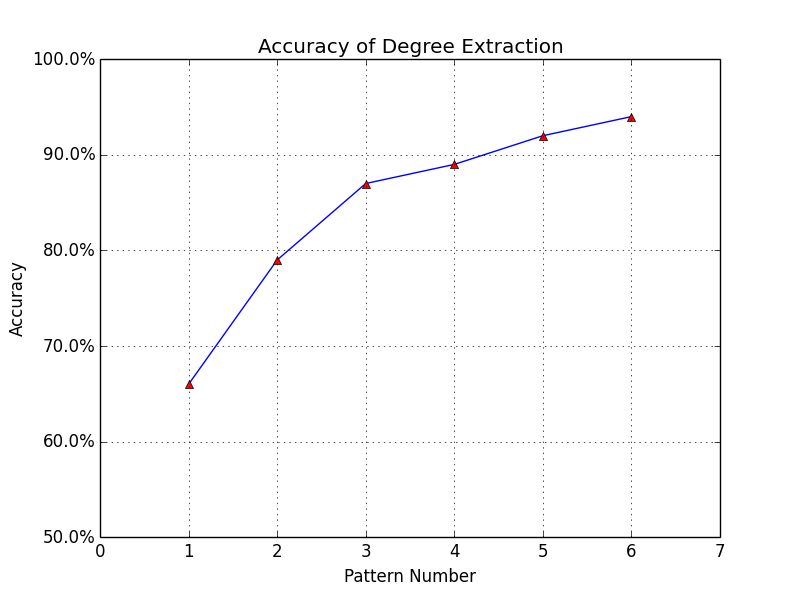
\includegraphics[scale=0.4]{images/degree_accuracy.png}
  \caption{Degree Extraction  Accuracy}
  \label{fig:degree_accuracy}
\end{figure}


\begin{table}[ht]
\caption{Information Extraction} % title of Table
\centering % used for centering table
\begin{tabular}{   | c | c | c | c |   }
 \hline
                     Field   & Pattern Num & Accuracy     \\
 \hline
                     Degree & 6         & 0.94          \\
 \hline
                     Major  & 10        & 0.85       \\
 \hline
                     Skill  & 6         & 0.82        \\
 \hline
\end{tabular}
\label{tab:ieaccura} % is used to refer this table in the text
\end{table}

\subsection{Experiments of Ontology Similarity}

From the table ~\ref{tab:dismatrix1} we got similarity value between skills. There is no standard criteria to measure the similarity of two entities.  To evaluate the accuracy of our result, we compare the result with human labeled data. We tested the two data sets.


\begin{table}
\small
\caption{Skills Similarity Table 1}
\begin{tabular}{ c | c c c c c c   }
 \hline
  Term       &  Java  &  JDBC  & Spring & Hibernate & MySql  & Oracle   \\  \hline
  Java   &   1    & 0.0523 & 0.091  &   0.0458  & 0.0339 & 0.0608    \\  \hline
    JDBC   & 0.0523 &   1    & 0.0525 &   0.0799  & 0.006  & 0.0616   \\  \hline
   Spring  & 0.091  & 0.0525 &   1    &   0.2008  & 0.0194 & 0.0878   \\  \hline
 Hibernate & 0.0458 & 0.0799 & 0.2008 &     1     & 0.0073 & 0.115    \\  \hline
   MySql   & 0.0339 & 0.006  & 0.0194 &   0.0073  &   1    & 0.049    \\
 \hline
   Oracle  & 0.0608 & 0.0616 & 0.0878 &   0.115   & 0.049  &   1      \\
 \hline
\end{tabular}
\label{tab:dismatrix1}
\end{table}

\begin{table}
\centering
\caption{ Javascript Similarity Evaluation : NDCG = 0.94 }
\begin{tabular}{ | c | c | c  | c |  }
 \hline
    Term     &  Similarity Value  &  Position   & Relevance     \\  \hline
    jQuery   &  0.1981            &      4      &   8        \\
     HTML    &  0.2087            &      3      &   4         \\
     CSS     &  0.2439            &      2      &   3   \\
     Java    &  0.0665            &      5      &   1   \\
    Python   &  0.0189            &      8      &   1   \\
     Ruby    &  0.023             &      7      &   1    \\
     JSP     &  0.0253            &      6      &   2    \\
 \hline
\end{tabular}
\label{tab:simcompare1}
\end{table}


\begin{table}
\centering
\caption{ HTML Similarity Evaluation : NDCG = 0.97 }
\begin{tabular}{ | c | c | c  | c |  }
 \hline
    Term      &  Similarity Value  &  Position   & Relevance     \\  \hline
  Javascript   &  0.2087           &      2      &   3        \\
     jQuery    &  0.0979           &      3      &   3         \\
     CSS     &  0.3569             &      1      &   5   \\
     Java    &  0.0473             &      4      &   1   \\
    Python   &  0.0175             &      6      &   1   \\
     Ruby    &  0.023              &      5      &   1    \\
     JSP     &  0.0103             &      7      &   3    \\
 \hline
\end{tabular}
\label{tab:simcompare2}
\end{table}





\subsection{Evaluation of the System}

To evaluate the system, some measures will be used. We also proposed two evaluation method: Pre-collected Data and User's direct experience.

In traditional information retrieval system, precision and NDCG are widely used measures ~\cite{manning2008introduction}.     Precision ($P$) is the fraction of retrieved documents that are relevant .
       $$  Precision =  \frac{ \#(releveant~items~ retrieved)}{ \#(retrieved~items)}$$

Since the results are ranked, $ Normalized~Discounted~Cumulative~Gain ( NDCG )$ will be an important measure to evaluate the ranked retrieval results. For a set of queries $Q$, let $R(j,d)$ be the relevance score assessors gave to document $d$ for query $j$.
       $$ NDCG(Q,k) = \frac {1}{|Q|} \sum_{j=1}^{|Q|}{Z_{kj}} \sum_{m=1}^{k} \frac{2^{R(j,m)} - 1}{ \log_2(1+m)} $$

where $Z_{kj}$ is a normalization factor calculated to make it so that a perfect ranking's NDCG at $k$ for query $j$ is 1. For queries for which $k' < k$ documents are retrieved, the last summation is done up to $k'$.


We collected some resumes from internet manually, and   job descriptions were collected by web crawler and stored in the database. In the evaluation phrase, we created a set of 100 job descriptions, which includes several kinds of jobs, like web developers, back-end developers, mobile developers and so on. The relevance value of job descriptions to each resume will be set manually. We would like to display jobs  that better match the candidate' resumes at the top. We create a query q from the resume, and treat the text of the job descriptions as documents d and apply standard ad-hoc retrieval techniques to rank the jobs.  The different retrieval algorithms we use are Okapi BM25~\cite{robertson2009probabilistic} ,   Kullback-Leibler divergence, and the TF-IDF. Since the job descriptions are fairly verbose we also experiment with a retrieval model where certain terms that are important to the quality of the match are weighted up in the TF-IDF scoring model.

\subsection{Experimental Results}

For our experiments to compare the various retrieval methods we used 8 candidate resumes  and retrieved the top 20 job descriptions  each method and judged the relevance of these against the resumes. The resumes we chose had an
average of 100 jobs per resume.  To compare performance of retrieval methods for the top results returned, we used
both Precision @ k e~\ref{tab:job_precision} and NDCG, shown in Table~\ref{tab:job_ndcg} . The result  shows that Ontology Similarity  performs the best. This agrees with results in  where it was found that finding and weighting
up important concepts in long queries can improve retrieval performance.

\begin{table}[ht]
\caption{Precision of Job Ranking } % title of Table
\centering % used for centering table
\begin{tabular}{    | c | c | c | c | c |  }
 \hline
       k     & Okapi BM25 & KL    & TF-IDF & Ontology Similarity  \\
 \hline
       5     & 0.13       & 0.40  & 0.54     & 0.74   \\
 \hline
       10    & 0.16       & 0.36  & 0.50     & 0.66   \\
 \hline
       20    & 0.16       & 0.35  & 0.49     & 0.61   \\
 \hline

\end{tabular}
\label{tab:job_precision} % is used to refer this table in the text
\end{table}


\begin{table}[ht]
\caption{NDCG of Job Ranking } % title of Table
\centering % used for centering table
\begin{tabular}{    | c | c | c | c | c |  }
 \hline
       k    & Okapi BM25 & KL    & TF-IDF & Ontology Similarity  \\
 \hline
       5    & 0.15       & 0.34  & 0.45     & 0.78   \\
 \hline
       10   & 0.18       & 0.44  & 0.47     & 0.72   \\
 \hline
       20   & 0.19       & 0.35  & 0.45     & 0.66   \\
 \hline

\end{tabular}
\label{tab:job_ndcg} % is used to refer this table in the text
\end{table}

\section{CONCLUSION and FUTURE WORK }
In this paper�� we described JobFinder a personalized job-resume matching system, which could help job seeker to find appropriate jobs more easily. The key technical components of the system are information extraction and ontology matching.

In the system, job descriptions and resumes will be processed by pipeline; and a finite automated tool will be used to extract the models from them. The models include fields like degree, major, skills.
To find the appropriate jobs, similarities between resume model and job description models will be calculated. The result will be sorted by the ontology similarity score, which is the sum of weighted multiple similarities of fields.

We proposed a finite automata matching library to matching the patterns in the sentences and extraction the information. We designed the a semi-automated algorithm to construct the domain specific ontology of skill set. To get the similarity between the skills, we proposed a statistical-based Ontology similarity measure.

Since finding a job is a complex process, which includes some subjective and objective factors.  Our work is just a initial work to solving  this problem, there are still a lof of parts could be improved.

First for the Information Extraction part, currently the method we used is pattern matching, we could try some machine learning approaches in future. In the resume model part, we could build more complex model, like resume model, which should consider the hiring history and project experience of of job seekers, and for job description model, the company's reputation and industry should be put into the model as well.


\bibliographystyle{acm-sigchi}
\bibliography{jobaly}
\end{document}
